\myChapter{Introduzione}
\section{Prefazione}
Lo scopo di questo elaborato è la riproduzione e lo studio di \textit{sketch-rnn} \cite{sketchrnn}: una rete neurale in grado di generare schizzi di semplici oggetti, composti da sequenze di tratti, appresi da un dataset di disegni creati da esseri umani. Il dataset è costantemente ampliato tramite \textit{Quick Draw!} \cite{quickdraw}, un gioco online in cui agli utenti viene chiesto di riprodurre alcuni oggetti entro 20 secondi, che al momento attuale costituisce la più vasta collezione di disegni al mondo. In questo lavoro viene proposta un'implementazione in \textit{Keras} \cite{keras}, un framework che a sua volta poggia su \textit{tensorflow} \cite{tensorflow}, che è la libreria software utilizzata per il lavoro originale.
\begin{figure}[ht]
	\centering
	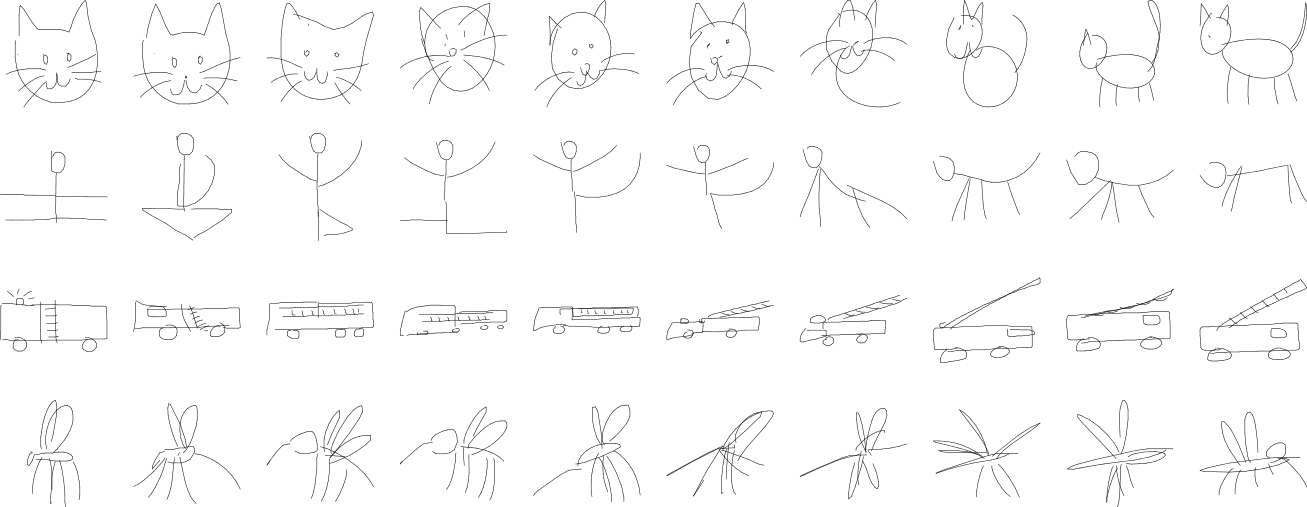
\includegraphics[width=\linewidth]{img/sketch_rnn_latent.png}
	\caption{Interpolazioni nello spazio di latenza di immagini vettoriali generate dal modello.}
	\label{fig:1.1}
\end{figure}
\section{Stato dell'arte}
Negli ultimi anni la generazione di immagini attraverso l'uso di reti neurali ha avuto ampia diffusione, fra i modelli più importanti possiamo citare: \textit{Generative Adversarial Networks (GANs)} \cite{GAN}, \textit{Variational Inference (VI)} \cite{VI} e \textit{Autoregressive Density Estimation (AR)} \cite{AR}. Il limite della maggior parte di questi algoritmi consiste nel fatto che lavorano con figure in pixel a bassa risoluzione, a differenza degli animali complessi che, piuttosto che vedere il mondo come una griglia di pixel, astraggono concetti per rappresentare ciò che osservano. Allo stesso modo degli esseri umani, che fin da piccoli imparano a riportare le proprie idee attraverso una sequenza di tratti su un foglio, questo modello generativo apprende da, e produce, immagini vettoriali.

L'obbiettivo è di addestrare una macchina a riprodurre ed astrarre concetti, in maniera analoga a come farebbe una persona. Ciò può avere numerose applicazioni in campo didattico come artistico, ad esempio assistendo il processo creativo, così come l'analisi della rappresentazione prodotta può offrire spunti di ricerca.
\section{Lavori correlati}

\section{Reti neurali}
Per spiegare le reti neurali e il Deep Learning si possono usare diversi approcci: si può ad esempio seguire il corso storico, introducendo il concetto di \textit{Percettrone}, passando ai Percettroni Multi-Strato ed ai primi metodi di ottimizzazione che furono applicati a questi modelli. Un'altra possibilità consiste nel partire da un punto di vista stocastico, definendo una regressione logistica che implica in modo naturale la minimizzazione di una \textit{loss function}. Ciò permette la definizione del concetto stesso di loss function e di come modificare dei parametri per ottenere una soluzione migliore, cosa che si ricollega perfettamente al concetto di Percettrone Multi-Strato come classificatore di una regressione logistica.

Di seguito verrà proposta la spiegazione di alcuni modelli fondamentali del Deep Learning, che saranno considerati come "mattoni" costitutivi della rete neurale studiata in questo progetto. Ciò aiuterà a comprendere agevolmente l'implementazione realizzata nel codice, seguendo un punto di vista coerente con le piattaforme più diffuse.
\section{Reti densamente connesse} % (fold)
\label{sec:reti_densamente_connesse}
Un neurone artificiale consiste in una funzione matematica che costituisce l'unità computazionale di base di una rete neurale artificiale.
\begin{figure}[ht]
	\centering
	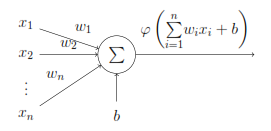
\includegraphics{img/artificial_neuron.PNG}
	\caption{Rappresentazione di un neurone artificiale.}
	\label{fig:1.2}
\end{figure}

Come si nota dalla figura \ref{fig:1.2} il neurone artificiale riceve \emph{n} input pesati $(w_1x_1,...,w_nx_n)$ e un bias \emph{b}. Successivamente li somma e applica una funzione non lineare nota come \textit{activation function} $\varphi$ per generare l'output. In sostanza calcolare l'output di un singolo neurone corrisponde a formare una combinazione lineare dei suoi input pesati e poi passarla ad una funzione di attivazione.

Per ragioni storiche, nel caso particolare in cui la funzione di attivazione consista di una funzione con una soglia lineare (e output binario), il neurone è detto \textit{Percettrone}.

Da qui in poi, quando ci riferiremo ad un \textit{layer} (strato) di una rete neurale staremo parlando di un raggruppamento di neuroni che formano, nello specifico, una colonna nel grafo della figura \ref{fig:1.2}, ovvero neuroni che si trovano allo stesso livello di profondità nella rete. Inoltre, ogni layer che si trova fra quello di input e quello di output verrà chiamato \textit{hidden layer}.

Come detto in precedenza, un Percettrone Multi-Strato (MLP da Multi-Layer Perceptron) può essere visto come un classificatore a regressione logistica dove l'input è trasformato utilizzando una trasformazione non lineare appresa $h(\boldsymbol{x})$ che costituisce l'hidden layer della nostra rete neurale (come in figura \ref{fig:1.2}). Questa trasformazione proietta l'input in uno spazio dove diventa linearmente separabile.

Questa computazione eseguita da una rete neurale multi-Strato, con un singolo hidden layer con una funzione di attivazione non lineare per elementi $\varphi_i$ sul vettore di input \textbf{x} e l'hidden output può essere scritta, in forma matriciale, come $\boldsymbol{y} = \varphi_2(W_2\varphi_1(W_1\boldsymbol{x} + \boldsymbol{b_1}) + \boldsymbol{b_2})$ dove $W_i, \boldsymbol{b_i}$ sono la matrice dei pesi e il vettore del bias dell'\textit{i}-esimo layer.

\begin{figure}[ht]
	\centering
	\begin{tikzpicture}[shorten >=1pt,->,draw=black!50, node distance=\layersep]
	    \tikzstyle{every pin edge}=[<-,shorten <=1pt]
	    \tikzstyle{neuron}=[circle,fill=black!25,minimum size=17pt,inner sep=0pt]
	    \tikzstyle{input neuron}=[neuron, fill=green!50];
	    \tikzstyle{output neuron}=[neuron, fill=red!50];
	    \tikzstyle{hidden neuron}=[neuron, fill=blue!50];
	    \tikzstyle{annot} = [text width=4em, text centered]

	    % Draw the input layer nodes
	    \foreach \name / \y in {1,...,3}
	    % This is the same as writing \foreach \name / \y in {1/1,2/2,3/3,4/4}
	        \node[input neuron, pin=left:Input \#\y] (I-\name) at (0,-\y) {};

	    \node[input neuron, pin=left:Input \#n] (I-4) at (0,-5) {};

	    % Draw the hidden layer nodes
	    \foreach \name / \y in {1,...,4}
	        \path[yshift=0.5cm]
	            node[hidden neuron] (H-\name) at (\layersep,-\y cm) {};

	    \node[hidden neuron] (H-5) at (\layersep,-5.5 cm) {};

	    % Draw the output layer node
	    \node[output neuron,pin={[pin edge={->}]right:Output}, right of=H-3] (O) {};

	    % Connect every node in the input layer with every node in the
	    % hidden layer.
	    \foreach \source in {1,...,4}
	        \foreach \dest in {1,...,5}
	            \path (I-\source) edge (H-\dest);

	    % Connect every node in the hidden layer with the output layer
	    \foreach \source in {1,...,5}
	        \path (H-\source) edge (O);

	    % Annotate the layers
	    \node[annot,above of=H-1, node distance=1cm] (hl) {Hidden layer};
	    \node[annot,left of=hl] {Input layer};
	    \node[annot,right of=hl] {Output layer};
	\end{tikzpicture}
	\caption{Rappresentazione di un modello Multi-Strato.}
	\label{fig:1.3}
\end{figure}

% \begin{figure}[ht]
% 	\centering
% 	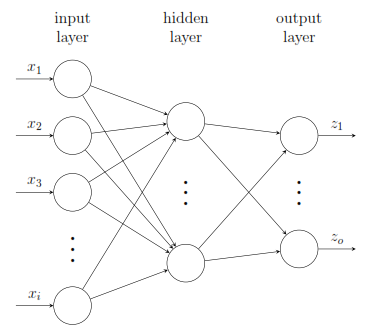
\includegraphics{img/MLN.png}
% 	\label{fig:1.3}
% \end{figure}

Seguendo il teorema di approssimazione universale \cite{approx} possiamo affermare che una rete neurale con un singolo hidden layer contenente un numero finito di neuroni (ovvero un MLP) è sufficiente per approssimare qualunque funzione continua su un sottoinsieme compatto di $\mathbb{R}^n$.

Alcuni sinonimi rilevanti utilizzati al posto di reti neurali Multi-Strato 
sono \textit{dense layers}, \textit{fully-connected layers} o, meno diffuso, \textit{inner product layers}.
% section reti_densamente_connesse (end)
\section{Reti ricorrenti}
\begin{figure}[ht]
	\centering
	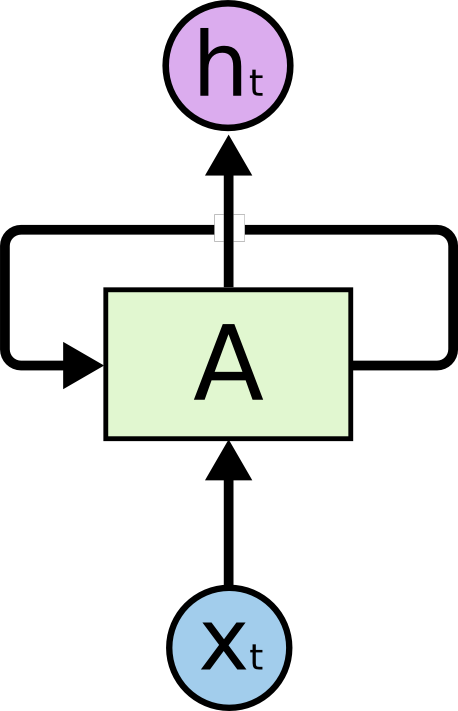
\includegraphics{img/RNN.png}
	\caption{Una semplice RNN (Recurrent Neural Network).}
	\label{fig:1.4}
\end{figure}
Il cervello umano, nello specifico il lobo frontale, è in grado di elaborare conseguenze future risultanti da azioni nel presente, ha la capacità di selezionare fra buone e cattive azioni (o fra migliori e ideali) e può determinare somiglianze e differenze fra oggetti ed eventi.

Molti problemi per essere risolti necessitano di un certo grado di conoscenza pregressa. Un esempio può riguardare le variazioni della luce di un semaforo: se, per esempio, si osserva che nel momento attuale la luce accesa è quella gialla, lo scopo sarebbe quello di sapere quale sarà la prossima ad accendersi. Le diverse posizioni delle luci in un semaforo sono irrilevanti: ciò che interessa sapere è quale colore apparirà, sapendo che quello appena apparso è il giallo. Nella maggior parte delle città è noto che la risposta sarebbe il rosso. Per rispondere a questa domanda è venuta in aiuto l'esperienza ma se si provasse a risolvere il problema utilizzando una rete neurale come quella proposta in precedenza non si otterrebbe una risposta soddisfacente. Ciò accade perché la soluzione presenta una dipendenza temporale, che corrisponde al metodo attraverso cui un essere umano apprende a risolvere problemi: analizzando sequenze di eventi.

Per trovare una soluzione a questo problema, com'è uso nel campo dell'Intelligenza Artificiale, si parte ancora una volta dai modelli basati sui principi biologici per elaborare una classe di reti neurali artificiali, in cui le connessioni fra le unità formano un ciclo orientato, dette Reti Neurali Ricorrenti (RNN da Recurrent Neural Networks, Fig. \ref{fig:1.4}). Queste connessioni creano uno stato interno della rete che le permette di esibire un comportamento dinamico nel tempo.

Per quanto riguarda le reti neurali non ricorrenti sono già state presentate molte conoscenze utili allo scopo di ottenere buoni parametri, di conseguenza si rende necessario trovare un modo di trasferire le potenzialità già discusse anche su questo nuovo tipo di reti neurali. Un'idea primitiva sarebbe quella di elaborare la rete ricorrente attraverso copie molteplici di una singola rete, come si vede in fig. \ref{fig:1.5}, trasferendo le informazioni dall'hidden layer \textit{A} alla copia successiva per realizzare una forma di memorizzazione.

\begin{figure}[ht]
	\centering
	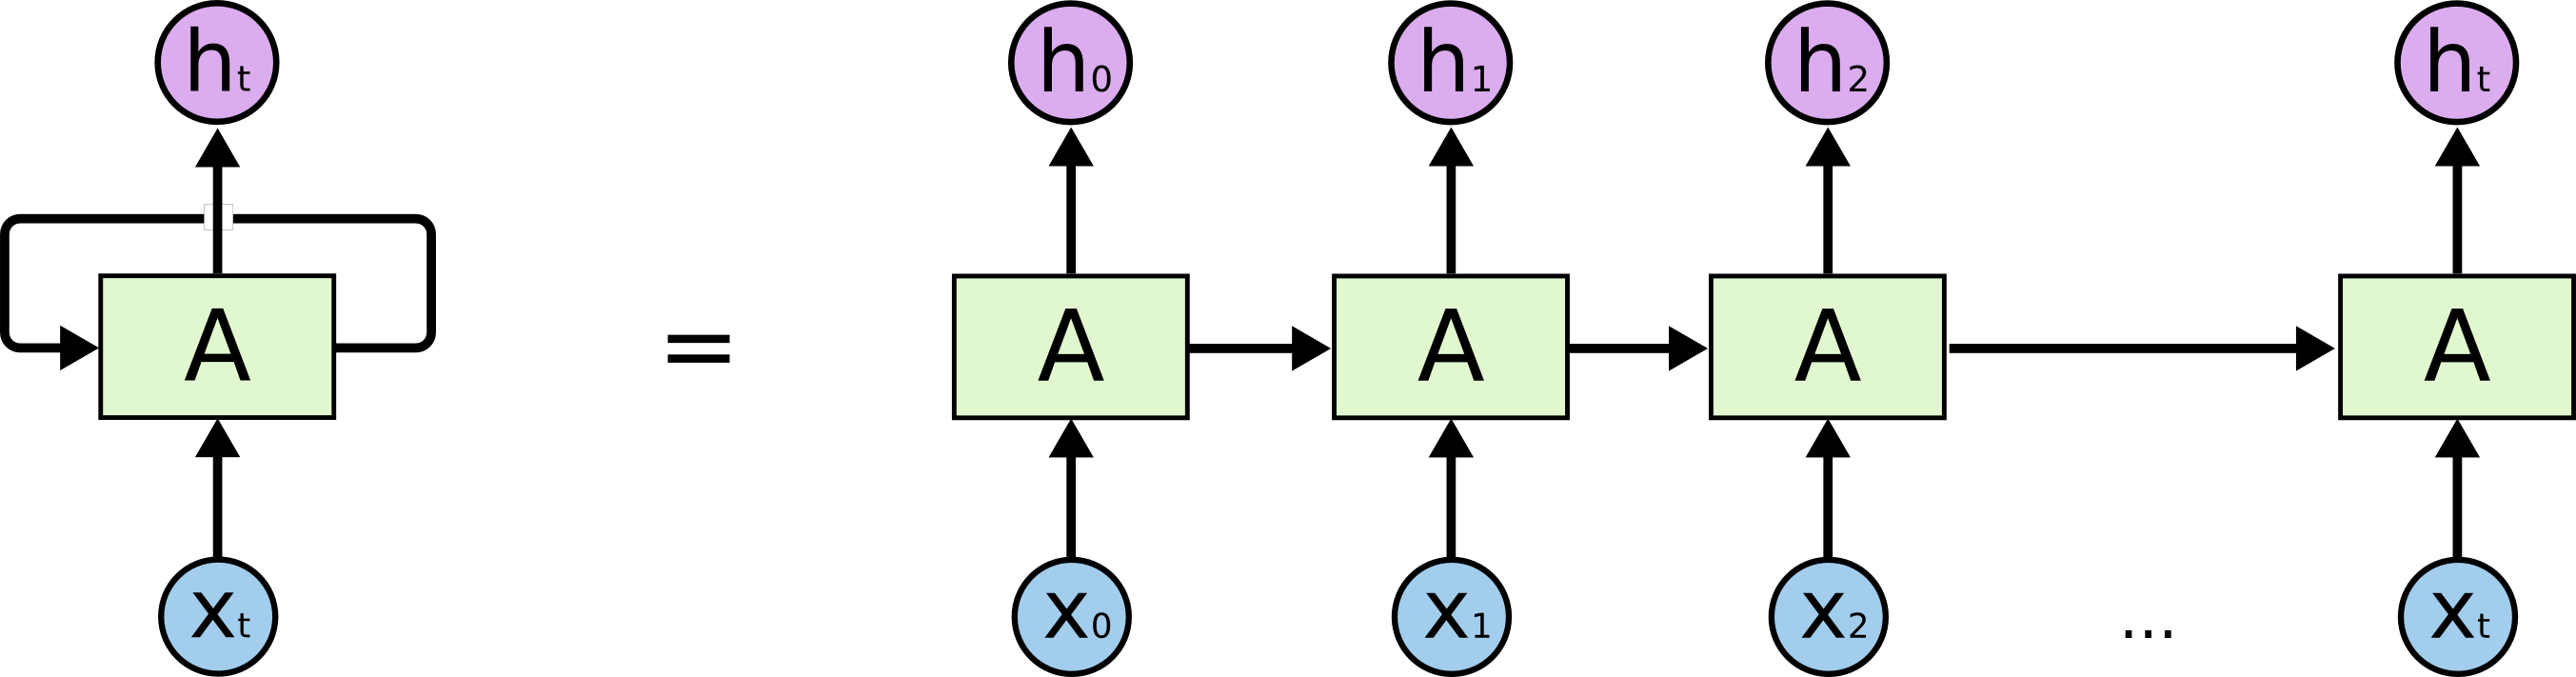
\includegraphics{img/unrolled_rnn.png}
	\caption{Una RNN dispiegata lungo la linea temporale.}
	\label{fig:1.5}
\end{figure}

Tuttavia ci potrebbero essere diversi modi di intendere la memoria e di combinare l'input del \textit{time-step} attuale con le informazioni ottenute dal precedente. Si prendono in considerazione due esempi: nel primo scegliamo di ottenere le informazioni precedenti conservando l'input, nel secondo l'hidden layer del time-step passato, ottenendo risultati completamente diversi. in fig. \ref{fig:1.6} sono riportati i due esempi sopra descritti, dove ogni colore rappresenta gli effetti sulla memoria dell'hidden layer \textit{A}.
\begin{figure}[ht]
	\centering
	\begin{tabular}{cc}
		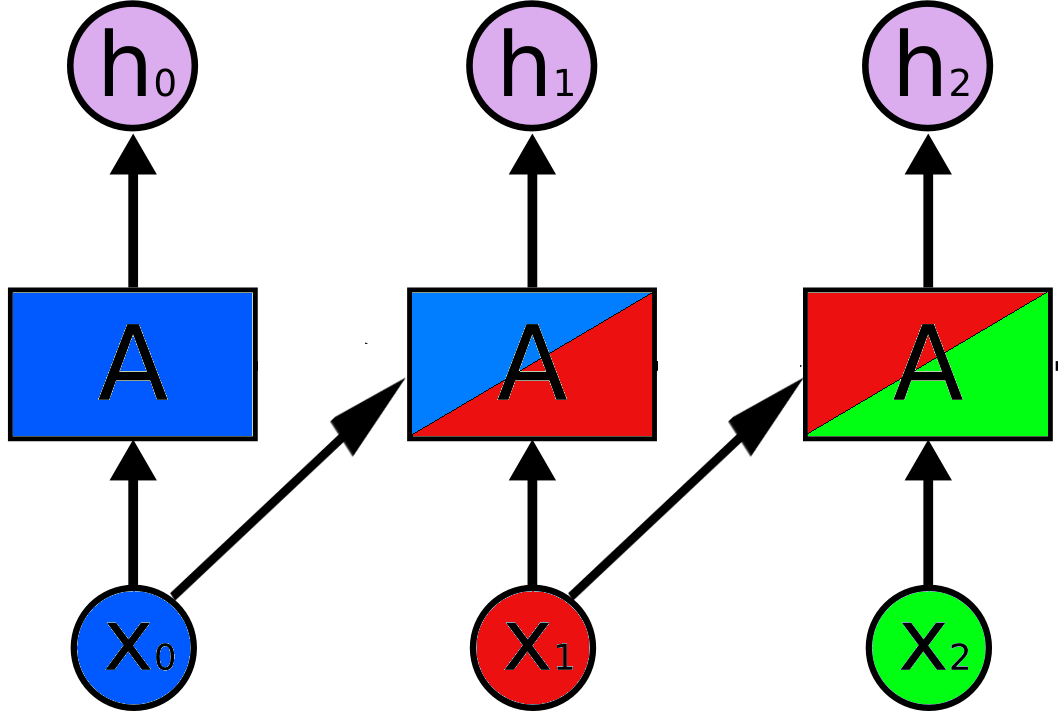
\includegraphics[width=0.4\linewidth]{img/input_memory.png} &
		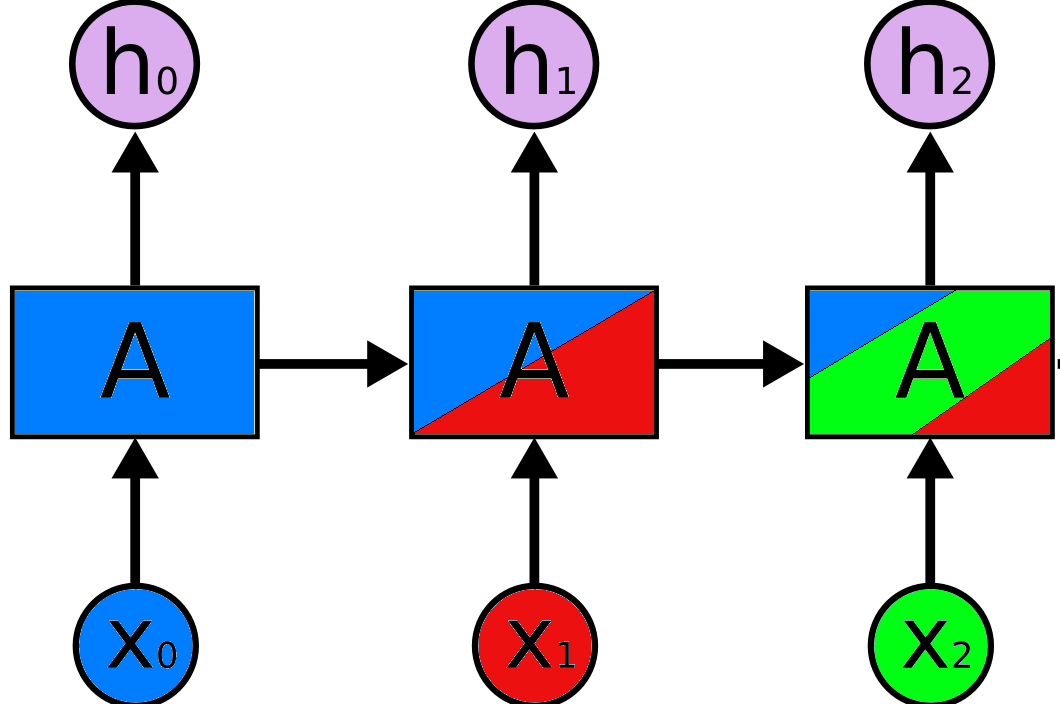
\includegraphics[width=0.4\linewidth]{img/hidden_memory.png} \\
		\footnotesize (a) Visualizzazione della memoria usando & \footnotesize (b) Visualizzazione della memoria usando \\ \footnotesize la ricorrenza dell'input & \footnotesize la ricorrenza dell'hidden layer
	\end{tabular}
	\caption{Due diversi metodi di implementazione della memoria in una RNN}
	\label{fig:1.6}
\end{figure}

Come si può vedere in fig. \hyperref[fig:1.6]{6(a)}, usando la ricorrenza dell'input viene ricordato solo l'attuale input e il precedente, invece nel caso della ricorrenza dell'hidden layer (fig. \hyperref[fig:1.6]{6(b)}) viene ricordata una mistura di tutti gli input precedenti. Per comprendere perché la seconda ipotesi è migliore si può usare questo esempio: si immagini di voler dedurre la parola seguente a \textit{"I love"} ("io amo") e che il testo contega le affermazioni \textit{"I love you"} ("ti amo") e \textit{"I love carrots"} ("amo le carote"). Se lo scopo è predire la decisione che verrà presa fra queste due opzioni e non sono note altre informazioni al di là dell'input (nel caso della ricorrenza dell'input), la rete neurale non avrà abbastanza informazioni per decidere. Viceversa, se la rete neurale possiede informazioni riguardanti il contesto, ad esempio se precedentemente si è parlato di cibo o di pasti, la sceltà diventerà più chiara. In teoria la ricorrenza dell'hidden layer può essere interpretata come un tentativo di ricordare ogni informazione con cui la rete neurale è entrata in contatto ma in pratica vige un limite tutt'al più di qualche passo.

Un'altra caratteristica delle RNN, che le avvantaggia ulteriormente rispetto alle MLN, è la versatilità. Le RNN, infatti, sono in grado di operare su sequenze di vettori, a differenza delle MLN o delle CNN (che non saranno trattate in questo elaborato) che operano su vettori di dimensioni fissate, così come fissato è il numero di passi computazionali (limitato ad esempio dal numero di hidden layers). Si possono elaborare sequenze sia in input che in output (o entrambi), in fig. \ref{fig:1.7} si distinguono cinque casi.
\newpage
\begin{figure}[ht]
	\centering
	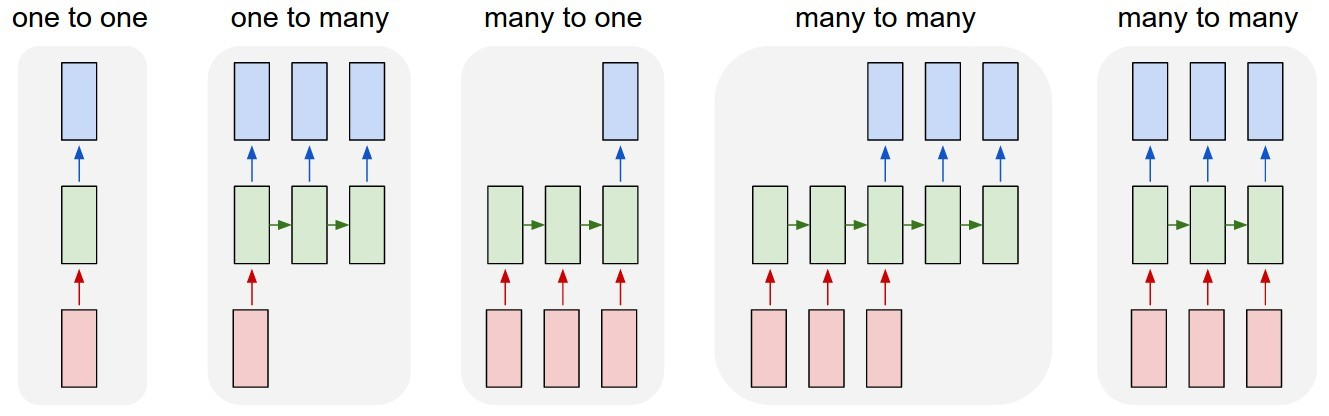
\includegraphics{img/rnn_seq.jpg}
	\caption{Combinazioni di sequenze vettoriali. \cite{rnn_effect}}
	\label{fig:1.7}
\end{figure}

\begin{enumerate}
	\item[Uno a uno:] il caso più semplice, in cui non vi è ricorrenza, ad esempio nella classificazione di immagini.
	\item[Uno a molti:] il caso in cui è presente una sequenza in output. Tipicamente usato nella creazione di sottotitoli, dove ad una sola immagine corrisponde una frase.
	\item[Molti ad uno:] in questo caso la sequenza è presente solo in input, è la struttura della \textit{sentiment analysis}, dove da una frase viene estratta la sensazione positiva/negativa contenuta in essa.
	\item[Molti a molti:] qui abbiamo una sequenza sia in input che in output, si potrebbe trattare di un modello di traduzione che assegna ad una frase in una lingua la frase corrispondente in un'altra.
	\item[Molti a molti (sinc.):] come nell'esempio precedente ma l'output è in sincronia con l'input. Utilizzato ad esempio nella classificazione video, in cui un'etichetta va assegnata ad ogni frame in tempo reale.
\end{enumerate}
\subsection{Dipendenze a lungo termine} % (fold)
\label{sub:dipendenze_a_lungo_termine}
\begin{figure}[ht]
	\centering
	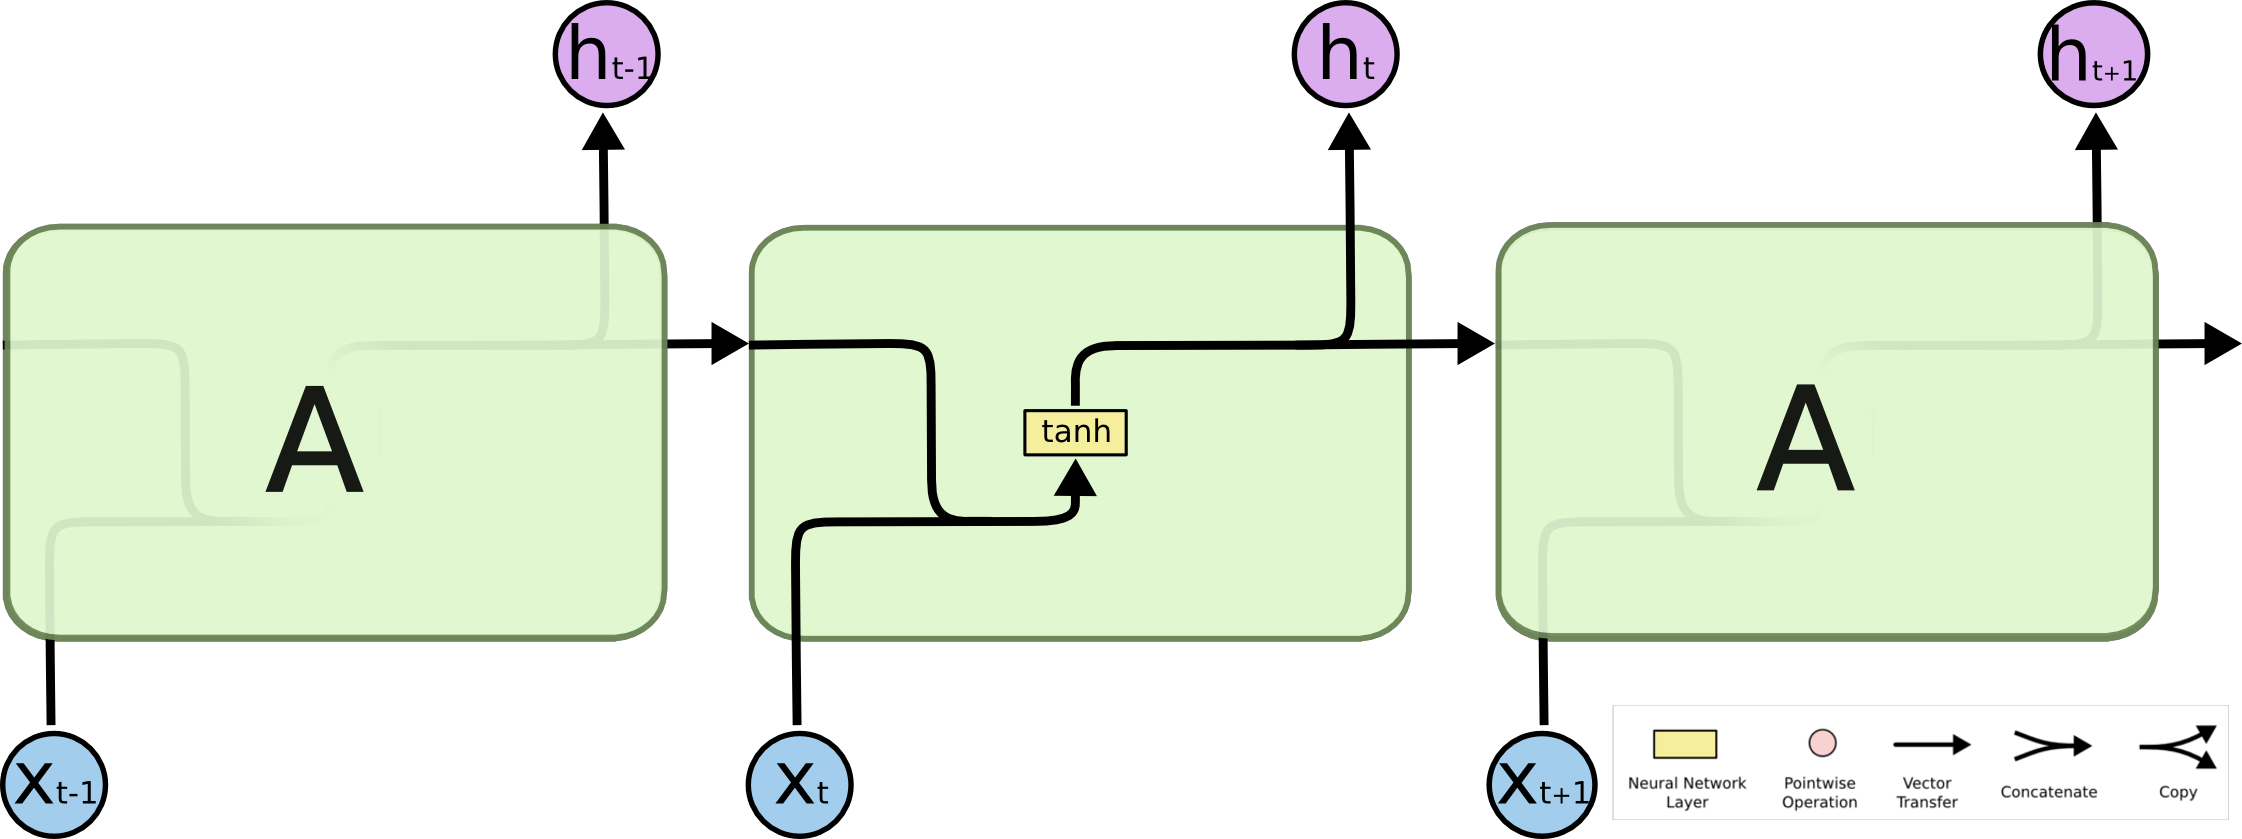
\includegraphics{img/rnn_struct.png}
	\caption{Struttura interna di una RNN standard con un singolo hidden layer.}
	\label{fig:1.8}
\end{figure}
Nel progettare una RNN va presa in considerazione la possibilità di incontrare la necessità di fornire un vasto numero di informazioni dal contesto per risolvere un problema. Tornando al compito della previsione di parole in un testo, si supponga di dover completare la frase "sto per andare a nuotare in", le informazioni a breve termine suggeriscono che la parola successiva sia un luogo dove sia possibile nuotare, sapendo che la frase precedente è "la spiaggia è molto assolata" si potrebbe dedurre che la parola da predire sia "mare". Il problema in questione è che si incontrano spesso difficoltà nell'identificare informazioni rilevanti. La formulazione di RNN data finora, in teoria, è perfettamente in grado di gestire dipendenze a lungo termine. In pratica, come spesso accade, si tratta di una prova tipicamente banale per una mente umana ma che una semplice implementazione (come in fig. \ref{fig:1.8}) non sarebbe in grado di risolvere efficacemente. Uno degli ostacoli più frequenti da risolvere è il cosiddetto problema del gradiente evanescente (\textit{vanishing gradient} \cite{vanishing}), per superarlo si rendono necessarie varianti più elaborate della RNN semplice, come le LSTM.
% subsection dipendenze_a_lungo_termine (end)
\subsection{Long Short Term Memory}
\begin{figure}[ht]
	\centering
	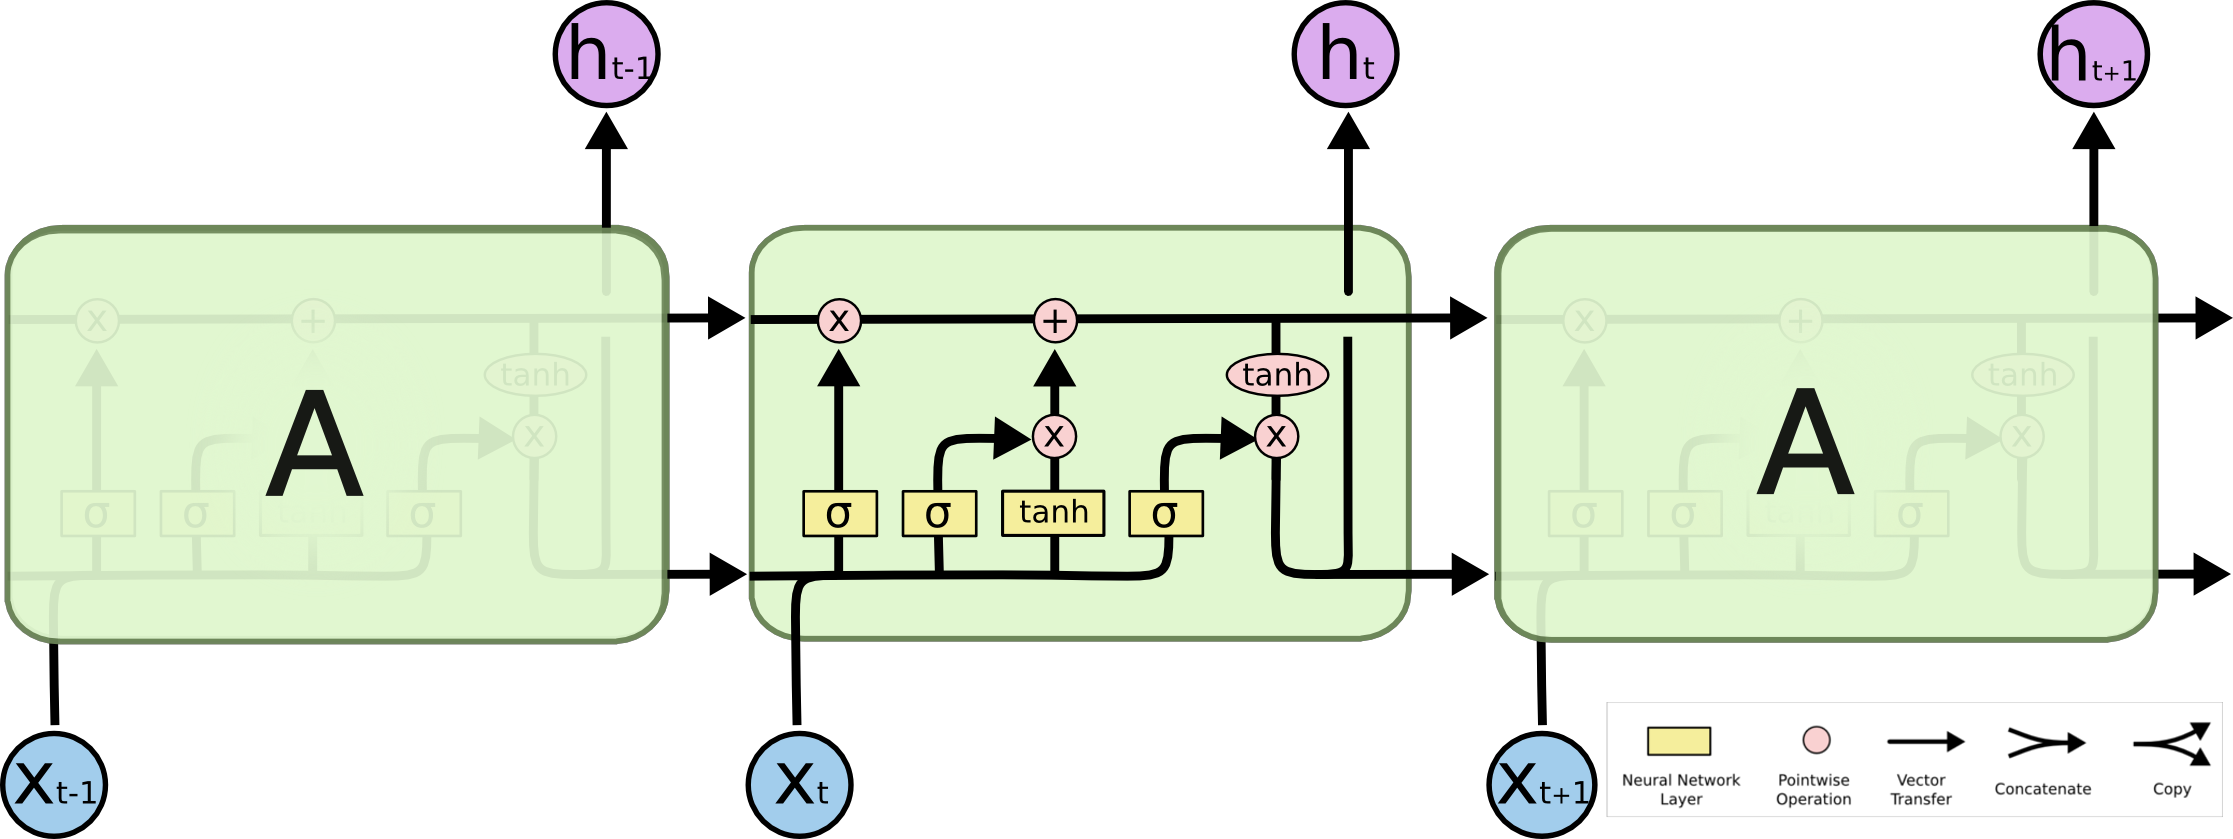
\includegraphics{img/lstm_struct.png}
	\caption{Struttura interna di una lstm che evidenzia i quattro strati interni di un layer}
	\label{fig:1.9}
\end{figure}
Per ottenere una RNN in grado di apprendere dipendenze a lungo termine, Hochreiter and Schmidhuber \cite{vanishing} introdussero, nel 1997, una versione detta \textit{Long Short Term Memory (LSTM)}.

A differenza di una RNN standard, che si limita ad una semplice struttura ripetuta, le LSTM operano una computazione complessa per ottenere lo stato interno. Invece della sola funzione di attivazione, una LSTM possiede strumenti per rimuovere, aggiungere o lasciar passare intatta l'informazione attraverso lo stato corrente del layer, detti \textit{gates} (cancelli). Questi gates sono composti da layer con attivazione sigmoide e operazioni di somma o moltiplicazione punto a punto, che definiscono quanto lasciar passare di ogni componente in ingresso.

Seguendo il diagramma in fig. \ref{fig:1.9}, vediamo in basso a sinistra il primo layer sigmoide, detto \textit{forget gate layer}, che si occupa di decidere quale informazione scartare dallo strato precedente o dall'input. Successivamente abbiamo il secondo layer sigmoide, detto \textit{input gate layer}, che decide quali valori saranno aggiornati, tramite l'output di un layer a tangente iperbolica. Questa combinazione va a modificare lo stato interno della LSTM, che attraversa la linea orizzontale superiore, che verrà poi trasferito allo stato successivo. Infine, dopo aver attraversato un'altra tangente iperbolica (per standardizzare i valori fra -1 e 1), un'altra sigmoide opera da gate per regolare l'output. \footnote{Esiste un'ampia varietà di modelli basati sulle LSTM, si suggeriscono: LSTM con "peephole connections" \cite{peephole} (connessioni a spioncino), Gated Recurrent Units (GRU) \cite{GRU} e Depth Gated RNNs \cite{DGRNN}}
\subsection{L'informazione futura} % (fold)
\label{sub:l_informazione_futura}
Per come sono state illustrate finora, le RNN si possono ritenere in grado di prendere in considerazione tutta l'informazione ricevuta fino al time frame corrente, dove la struttura specifica della rete e l'algoritmo utilizzato per l'apprendimento definiscono quanta di questa informazione verrà effettivamente sfruttata.

Talvolta accade che, allo scopo di migliorare la previsione corrente, si renda utile conoscere anche una parte dell'informazione successiva a quella dell'attuale time frame (ad esempio il genere del soggetto di una frase, nel determinare la traduzione di un articolo da una lingua con articoli neutri ad un'altra). La generica RNN potrebbe ottenere questo risultato aggiungendo un ritardo sull'output di un certo numero \textit{M} di time frames, per includere l'input fino a $\boldsymbol{x}_{t_c + M}$ allo scopo di predire $\boldsymbol{y}_{t_c}$. In teoria \textit{M} potrebbe essere scelto largo abbastanza da includere tutto l'input restante, in pratica empiricamente è noto che la bontà della previsione diminuisce drasticamente per un \textit{M} troppo grande. Una possibile spiegazione a questo potrebbe essere che al crescere di \textit{M} le capacità predittive della rete si vadano sempre più concentrando nel ricordare l'input fino a $\boldsymbol{x}_{t_c + M}$, lasciando sempre meno potenza di elaborazione per combinare le conoscenze da diversi vettori.

Nonostante quest'operazione di ritardo di alcuni frames sia stata concretamente sfruttata con successo per migliorare i risultati in un sistema di riconoscimento vocale \cite{phone}, successo confermato anche da esperimenti indipendenti \cite{BRNN}, il ritardo ottimale dipende dal compito specifico ed è stato ottenuto con prove ed errori sul validation set. Sarebbe naturalmente preferibile un approccio più elegante.

Per sfruttare tutta l'informazione disponibile, è possibile usare due diverse reti (una per ogni direzione) e in qualche modo combinare i loro risultati. Entrambe le reti possono essere considerate esperte del problema specifico su cui sono state addestrate. Un modo per combinare le \textit{"opinioni di esperti"} è di assumerne l'indipendenza, che comporta l'uso della media aritmetica per la regressione e della media geometrica (o, alternativamente, la media aritmetica nel dominio logaritmico) per la classificazione. Queste procedure sono dette \textit{linear opinion pooling} e \textit{logarithmic opinion pooling} rispettivamente \cite{SDT}, \cite{combining}. Nonostante la semplice combinazione degli output sia stata applicata con buoni risultati \cite{phone1}, non è chiaro, in generale, come effettuarla efficacemente, dal momento che reti diverse addestrate sugli stessi dati non possono essere considerate effettivamente indipendenti.
\begin{figure}[ht]
	\centering
	
\includegraphics[width=\linewidth]{img/rnn_confront.png}
	\caption{Confronto sull'utilizzo dell'input in diverse reti neurali.}
	\label{fig:1.10}
\end{figure}
% subsection l_informazione_futura (end)
\subsection{Reti bidirezionali}
Allo scopo di superare le limitazioni di una generica RNN, esposte nella sezione precedente, è stata ideata una struttura detta \textit{Bidirectional Recurrent Neural Network} (BRNN, rete neurale ricorrente bidirezionale) che può essere addestrata con tutte le informazioni in input, passate e future, di ogni time frame.
\begin{figure}[ht]
	\centering
	
\includegraphics[width=\linewidth]{img/BRNN.png}
	\caption{Struttura generica di una BRNN, svolta lungo tre time steps.}
	\label{fig:1.11}
\end{figure}

L'idea alla base della BRNN è quella di suddividere lo stato interno di un elemento di una RNN regolare in due parti: una responsabile per la dimensione temporale positiva (forward), una per quella negativa (backward). Gli output dagli stati forward non sono connessi agli input di quelli backward e viceversa. Ciò conduce alla struttura che si può vedere in fig. \ref{fig:1.11}.
Si può notare come eliminando gli stati backward, questa struttura diventa analoga a quella di una generica RNN come in fig. \ref{fig:1.5}. Rimuovendo gli stati forward, invece, otteniamo una RNN con l'asse temporale invertito. Prendere in considerazione entrambe le direzioni temporali, rende possibile utilizzare direttamente tutta l'informazione passata e futura rispetto al time step corrente, senza alcun bisogno di ricorrere a ritardi.

Una BRNN può essere addestrata con gli stessi algoritmi con cui si addestrerebbe una RNN semplice, dal momento che non vi sono interazioni fra le due tipologie di stati e, di conseguenza, può essere svolta in una generica rete ad avanzamento semplice. Tuttavia se, ad esempio, viene utilizzata una forma qualunque di \textit{back propagation through time} (BPTT), la procedura del passo forward e backward diventa leggermente più complessa, dal momento che l'aggiornamento dello stato e dell'output non può più essere effettuato uno per volta. In questo caso, i passi forward e backward lungo la BRNN svolta lungo il tempo vengono effettuati all'incirca allo stesso modo che per un MLP regolare. Alcuni accorgimenti particolari sono richiesti solo all'inizio e alla fine dei dati di addestramento\footnote{Si rimanda a \cite{BRNN} per approfondimenti e varianti.}.
%\section{Reti autoregressive}
\section{Autoencoder}
\begin{figure}[ht]
	\centering
	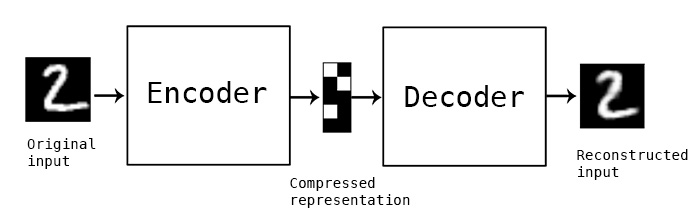
\includegraphics[width=0.8\linewidth]{img/autoencoder_schema.jpg}
	\caption{Struttura di un generico AutoEncoder, da \cite{keras_blog}}
	\label{fig:1.12}
\end{figure}
Il processo di \textit{autoencoding} indica il risultato di un algoritmo di compressione, dove le funzioni di compressione e decompressione presentano le seguenti caratteristiche: sono specifiche dei dati, presentano perdite e sono apprese automaticamente attraverso gli esempi, piuttosto che codificate a mano da un programmatore. L'ultima di queste caratteristiche rimanda immediatamente all'uso di una rete neurale, che infatti è l'implementazione tipica di un autoencoder.

A differenza degli algoritmi di compressione genericamente utilizzati, ad esempio MPEG-2 Audio Layer III (comunemente detto MP3) per l'audio, che si prestano ad un utilizzo ampio, un autoencoder è limitato dal dataset su cui viene addestrato. Le prestazioni su un autoencoder addestrato su di un certo suono o su fotografie di volti crollerebbero drasticamente, su suoni diversi o su fotografie di alberi. Allo stesso modo di alcuni degli algoritmi più comuni, l'output dopo la decompressione presenta una diminuzione di qualità rispetto all'input originale. In compenso è facile addestrare istanze specifiche dell'algoritmo, che presentino buoni risultati su un particolare input, in quanto non sono generalmente necessari nuovi interventi di ingegneria del software ma solo dati appropriati.

Per assemblare un autoencoder sono necessarie tre componenti fondamentali: una funzione che operi la codifica, una che operi la decodifica e una che misuri la distanza che occorre fra la rappresentazione compressa e quella ottenuta dalla ricostruzione, in termini di perdita di dati (ovvero una loss function).
Decoder ed encoder (fig \ref{fig:1.12}) sono tipicamente funzioni parametriche (reti neurali), differenziabili rispetto alla funzione di distanza in modo da essere ottimizzabili per minimizzare la perdita in ricostruzione, usando lo \textit{Stochastic Gradient Descent} (SGD).
\section{Modelli Generativi} % (fold)
\label{sec:modelli_generativi}
All'inizio di questo elaborato è stato citato brevemente il concetto di \textit{modello generativo}, poi ripreso in alcuni esempi nella sezione riguardante le reti ricorrenti.

Gli algoritmi finora elencati, nella loro implementazione più semplice, formano modelli che tipicamente stabiliscono i confini che intercorrono fra le varie classi a cui possono appartenere i dati in input. Per questa ragione sono detti \textit{modelli discriminativi}, in quanto non si preoccupano di fare assunzioni sull'origine dei dati forniti ma si limitano a categorizzarli nel modo più efficace. Lo scopo di un modello generativo, invece, è quello di apprendere come sono stati generati i dati ottenuti, producendo una rappresentazione delle classi a cui appartengono attraverso l'analisi delle caratteristiche rilevate nell'input.

Da un punto di vista matematico, un modello discriminativo cerca di apprendere la distribuzione di probabilità condizionata rispetto ai dati, in formule: 
\begin{equation}
	\label{conditional}
	f(\boldsymbol{x}) = arg \max_y p(\boldsymbol{y}|\boldsymbol{x})
\end{equation}
Per contro, un modello generativo cerca di apprendere la distribuzione di probabilità congiunta, ovvero, usando la regola di Bayes (e liberandoci di $p(x)$, in quanto massimiziamo secondo $y$):
\begin{equation}
	\label{joint}
	f(\boldsymbol{x}) = arg\max_y p(\boldsymbol{y}|\boldsymbol{x})p(\boldsymbol{y})
\end{equation}
Che corrisponde a $p(x, y)$. Come si può notare intuitivamente, ad un modello generativo è richiesta una complessità superiore che si può tradurre in un calo di prestazioni su compiti meno elaborati, rispetto ai modelli discriminativi, ad esempio nella classificazione. D'altra parte un modello discriminativo non è in grado di cogliere caratteristiche e relazioni complesse fra i dati in input e le variabili target, né è in grado di produrre dati originali analoghi a quelli appresi, proprietà che rendono preferibile un modello generativo per compiti di apprendimento non supervisionato e che sono fondamentali per generare astrazioni come quelle ricercate nella riproduzione di disegni a mano.
% section modelli_generativi (end)
\section{Variabili latenti} % (fold)
\label{sec:variabili_latenti}
Una variabile latente è una variabile casuale che condiziona la generazione dell'output di un modello. Se, ad esempio, si volessero generare immagini di cifre scritte a mano (database MNIST), se nella metà sinistra della cifra è presente metà del carattere \textit{5}, non si può accettare che nella metà destra compaia metà del carattere \textit{0}. In questo caso, la variabile latente permette di stabilire in precedenza quale carattere generare, prima di assegnare valori ai pixel. La variabile è detta \textit{latente} poiché dato il carattere prodotto dal modello non si possiede necessariamente l'informazione su quale assetto della variabile l'abbia generato. 

Prima di poter dire che un modello è in grado di rappresentare il dataset considerato per ogni punto $\boldsymbol{x}$, ci si deve assicurare che esista un assetto della variabile latente che permette al modello di generare un punto molto simile ad esso. Formalmente si supponga di avere un vettore di variabili latenti $\boldsymbol{z}$, in uno spazio multidimensionale $\boldsymbol{Z}$ che si può facilmente campionare in accordo ad una qualche funzione di densità di probabilità (PDF - Probability Density Function) $P(\boldsymbol{z})$ definita su $\boldsymbol{Z}$. Successivamente, si supponga di avere una famiglia di funzioni deterministiche $f(\boldsymbol{z}, \boldsymbol{\theta)}$, parametrizzate rispetto ad un vettore $\boldsymbol{\theta}$ su di un qualche spazio $\boldsymbol{\Theta}$, dove $f : \boldsymbol{Z} x \boldsymbol{\Theta} \rightarrow \boldsymbol{\chi}$. $f$ è deterministica ma, se $\boldsymbol{z}$ è casuale e $\boldsymbol{\theta}$ è fissato, allora $f(\boldsymbol{z}; \boldsymbol{\theta})$ è una variabile casuale nello spazio $\boldsymbol{\chi}$. Si desidera ottimizzare $\boldsymbol{\theta}$ in modo da poter campionare $\boldsymbol{z}$ da $P(\boldsymbol{z})$ e, con alta probabilità, $f(\boldsymbol{z}; \boldsymbol{\theta})$ sarà analoga alle $\boldsymbol{x}$ del dataset considerato.

In modo matematicamente rigoroso, si può affermare che l'obbiettivo è massimizzare la probabilità di ogni $\boldsymbol{x}$ nel training set lungo tutto il procedimento generativo, in accordo a:
\begin{equation}
	\label{probability}
	P(\boldsymbol{x}) = \int P(\boldsymbol{x} | \boldsymbol{z}; \boldsymbol{\theta}) P(\boldsymbol{z})d\boldsymbol{z}
\end{equation}

Qui $f(\boldsymbol{z}, \boldsymbol{\theta)}$ è stato rimpiazzato da $P(\boldsymbol{x} | \boldsymbol{z}; \boldsymbol{\theta})$, che permette di rendere esplicita la dipendenza di $\boldsymbol{x}$ da $\boldsymbol{z}$ attraverso la regola delle probabilità totali. L'intuizione dietro a questo framework, detto \textit{"maximum likelihood"}, è che se il modello è in grado di riprodurre esempi del training set, sarà probabilmente in grado di generare esempi analoghi e con poca probabilità produrrà risultati molto diversi.
% section variabili_latenti (end)
\section{Variational Autoencoder}
\begin{figure}[ht]
	\centering
	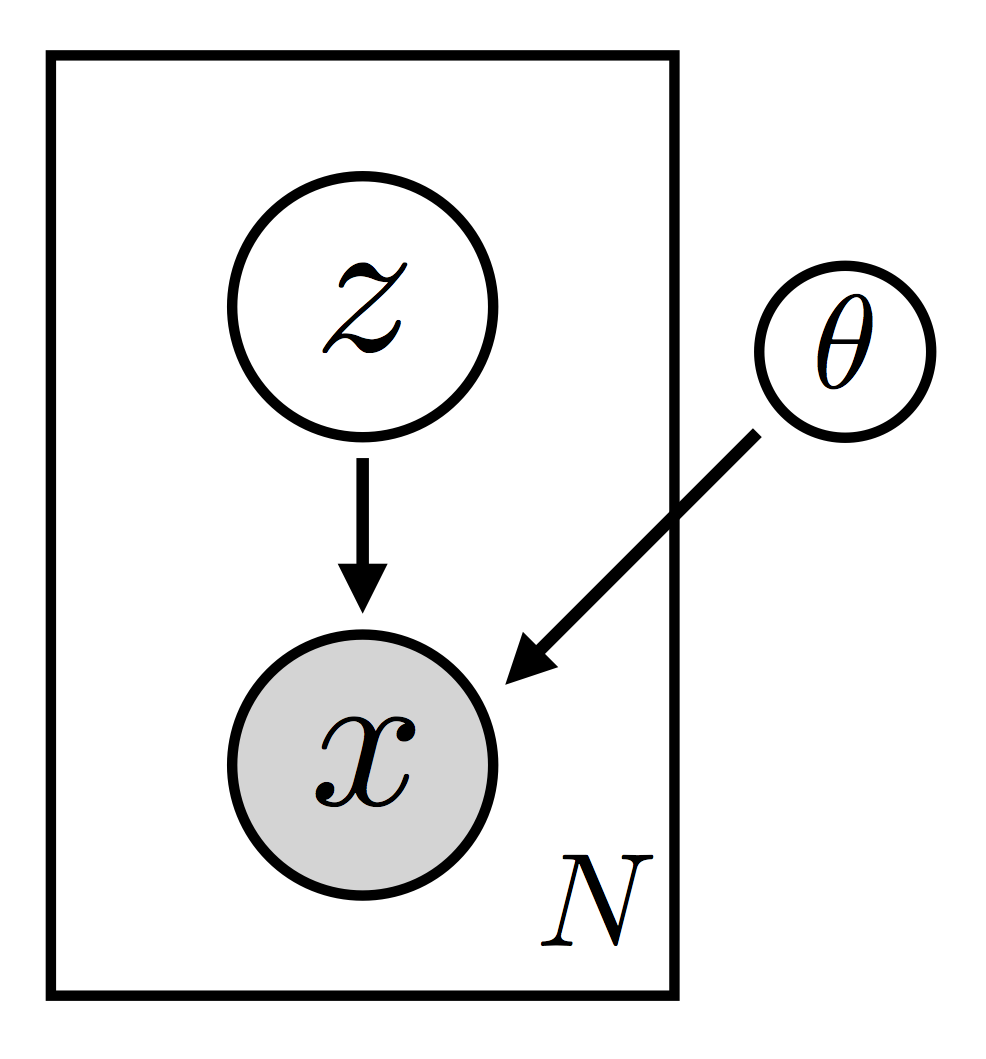
\includegraphics[width=0.4\textwidth]{img/vae_model.png}
	\caption{Modello di un VAE}
	\label{fig:1.13}
\end{figure}
I variational autoencoder realizzano l'implementazione di un modello generativo attraverso una struttura analoga a quella degli autoencoder tradizionali, seppur fondandosi su principi matematici diversi, per la presenza di un encoder ed un decoder nella propria struttura. Si tratta di una classe di modelli che si basano sulla generazione condizionata da una variabile latente.

Nei VAE, la scelta della distribuzione di output è spesso gaussiana, ovvero della forma:
\begin{equation}
	\label{gaussian_probability}
	P(\boldsymbol{x} | \boldsymbol{z}; \boldsymbol{\theta}) = \mathcal{N}(\boldsymbol{x}|f(\boldsymbol{z}; \boldsymbol{\theta}), \sigma^2 * \boldsymbol{I})
\end{equation}
Il che significa che ha media $f(\boldsymbol{z}; \boldsymbol{\theta})$ e covarianza pari alla matrice identità moltiplicata per un qualche scalare $\sigma$ (che è un iperparametro). In ogni caso ciò non è obbligatorio, ad esempio, se $\boldsymbol{x}$ fosse binario, allora $P(\boldsymbol{x} | \boldsymbol{z})$ potrebbe essere una distribuzione di Bernoulli parametrizzata da $f(\boldsymbol{z}; \boldsymbol{\theta})$. La proprietà fondamentale è che $P(\boldsymbol{x} | \boldsymbol{z})$ sia computabile e continua in $\theta$.

Per risolvere questa equazione, ci sono due problemi che i VAE devono affrontare: come definire la variabile latente $\boldsymbol{z}$ (ovvero decidere quale informazione debba rappresentare) e come gestire l'integrale lungo $\boldsymbol{z}$.

La necessità fondamentale della variabile latente è quella di rappresentare il più accuratamente possibile l'informazione latente. Dovendo ad esempio rappresentare delle cifre scritte a mano (MNIST) dovrebbe non solo determinare quale cifra rappresentare ma anche l'angolo con cui disegnarla, lo spessore del tratto ed altre proprietà prettamente stilistiche. A complicare le cose c'è il fatto che queste proprietà potrebbero presentare dipendenze: una cifra maggiormente inclinata potrebbe essere correlata ad una scrittura più frettolosa e, di conseguenza, ad un tratto più sottile. Idealmente si vorrebbe evitare di stabilire manualmente quali informazioni verranno codificate in ogni dimensione di $\boldsymbol{z}$, inoltre sarebbe da evitare anche la descrizione specifica delle dipendenze fra le dimensioni. L'approccio sfruttato dai VAE è inusuale: partono dall'assunto che non ci sia un'interpretazione semplice delle dimensioni, affermando che campioni di $\boldsymbol{z}$ possano essere estratti piuttosto da una distribuzione semplice, ovvero $\mathcal{N}(0, \boldsymbol{I})$. La chiave di questa logica sta nell'osservare che una distribuzione qualunque in \textit{d} dimensioni, può essere generata attraverso un set di \textit{d} variabili casuali con distribuzione normale, mappante tramite una funzione sufficientemente complicata\footnote{In una dimensione si può utilizzare l'inversa della funzione a distribuzione cumulativa (CDF - cumulative distribution function) della distribuzione desiderata, composta con la CDF di una Gaussiana, in estensione al principio di \textit{"inverse transform sampling"}. Per dimensioni multiple si può applicare il medesimo processo cominciando con la distribuzione marginale di una dimensione e ripetendo con quella condizionale di ogni dimensione aggiuntiva. Si veda "inversion method" e "conditional distribution method" in Devroye et al. \cite{rvg}}.
\section{MDN}
\subsection{Misture gaussiane} % (fold)
\label{sub:misture_gaussiane}

% subsection misture_gaussiane (end)